\documentclass[tikz,border=8pt]{standalone}
% Shared look for every TikZ diagram. Load with \input{../../tools/tikz-style.tex}
\usepackage[T1]{fontenc}
\usepackage{lmodern}
\renewcommand{\sfdefault}{lmr}  % diagrams use the same serif as the text
\usetikzlibrary{arrows.meta, positioning, shapes.geometric, calc, fit, backgrounds}
\definecolor{cblue}{HTML}{4C78A8}
\definecolor{corange}{HTML}{F58518}
\definecolor{cgreen}{HTML}{54A24B}
\definecolor{cred}{HTML}{E45756}
\definecolor{cpurple}{HTML}{B279A2}
\definecolor{cgrey}{HTML}{6B6B6B}
\tikzset{
  every picture/.style={font=\sffamily, line width=1.2pt},
  box/.style={draw=#1, fill=#1!12, rounded corners=4pt, align=center, inner sep=7pt, minimum height=1.1cm},
  box/.default=cgrey,
  arrow/.style={-{Stealth[length=3mm]}, draw=cgrey, line width=1.4pt},
  title/.style={font=\sffamily\bfseries\Large},
  note/.style={font=\sffamily\small, text=cgrey, align=center},
}
\AtBeginDocument{\hyphenpenalty=10000 \exhyphenpenalty=10000}

\begin{document}
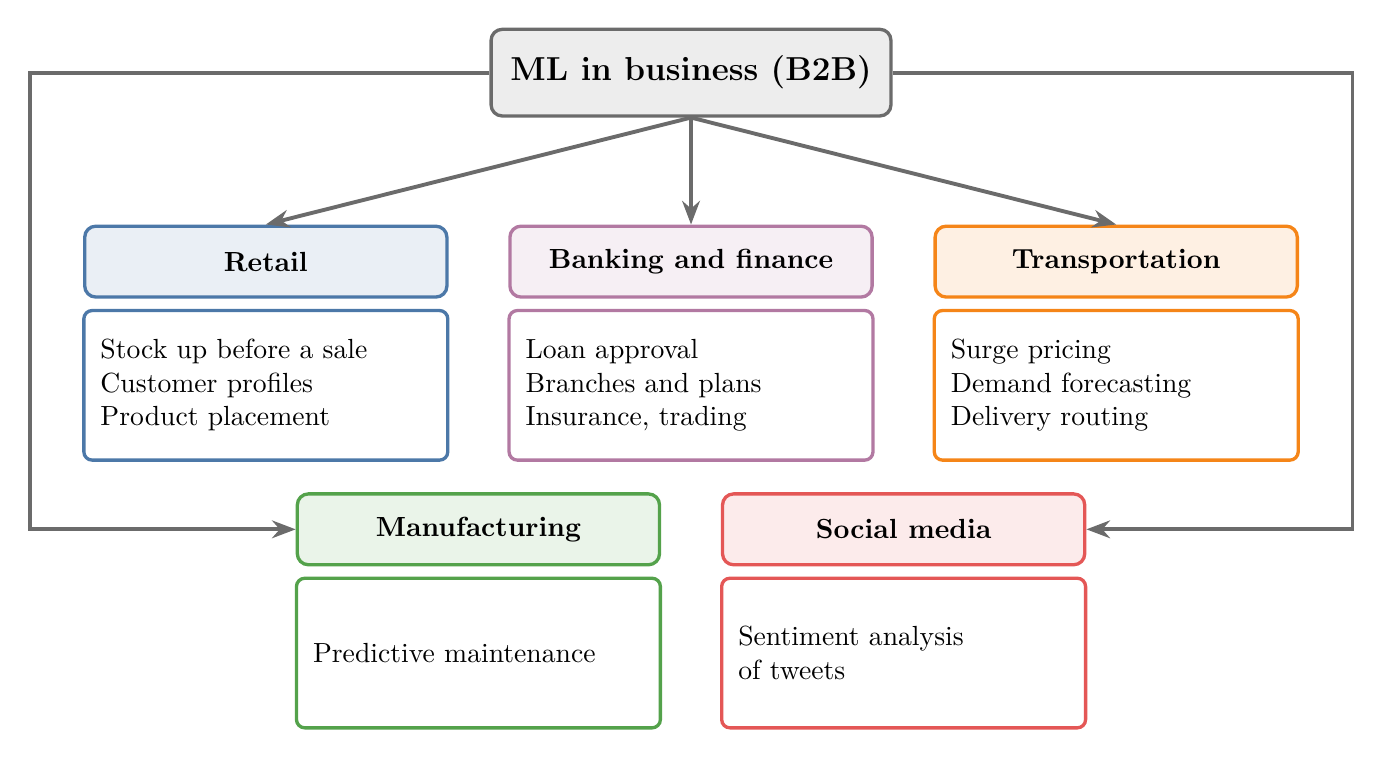
\begin{tikzpicture}
  \tikzset{sector/.style={box=#1, minimum width=4.6cm, minimum height=0.9cm, font=\bfseries},
           app/.style={draw=#1, fill=white, rounded corners=3pt, align=left, inner sep=6pt,
                       text width=4.2cm, minimum height=1.9cm, anchor=north}}
  \newcommand{\sector}[5]{% id, colour, x, y, name ; apps given after
    \node[sector=#2] (#1) at (#3,#4) {#5};}
  \node[box=cgrey, minimum width=5cm, font=\bfseries\large] (ml) at (5.4,2.4) {ML in business (B2B)};
  \sector{r}{cblue}{0}{0}{Retail}
  \node[app=cblue] at (0,-0.6) {Stock up before a sale\\Customer profiles\\Product placement};
  \sector{b}{cpurple}{5.4}{0}{Banking and finance}
  \node[app=cpurple] at (5.4,-0.6) {Loan approval\\Branches and plans\\Insurance, trading};
  \sector{t}{corange}{10.8}{0}{Transportation}
  \node[app=corange] at (10.8,-0.6) {Surge pricing\\Demand forecasting\\Delivery routing};
  \sector{m}{cgreen}{2.7}{-3.4}{Manufacturing}
  \node[app=cgreen] at (2.7,-4.0) {Predictive maintenance};
  \sector{s}{cred}{8.1}{-3.4}{Social media}
  \node[app=cred] at (8.1,-4.0) {Sentiment analysis\\of tweets};
  \foreach \n in {r,b,t} \draw[arrow] (ml.south) -- (\n.north);
  \draw[arrow] (ml.west) -| (-3.0,-3.4) -- (m.west);
  \draw[arrow] (ml.east) -| (13.8,-3.4) -- (s.east);
\end{tikzpicture}
\end{document}
